\chapter{Switching MM}\label{chap:smm}

The previous chapters read the Collatz iteration as an optimization method:
the odd step is an injection that raises the potential $\log x$, the halvings
are the corrective descent, and \cref{chap:momentum} made precise how far the
analogy with accelerated gradient methods can be pushed before it breaks. In
this chapter and the next we run the analogy in the opposite direction. We
take two pieces of the arithmetic, a single number and a parity pattern, and
build from them an ordinary first order method for smooth optimization. The
method is called Switching MM\index{Switching MM}, abbreviated SMM. It uses the momentum\index{momentum}
coefficient
\[
  \beta \;=\; \frac{\log(3/2)}{\log 2} \;=\; \lt-1 \;\approx\; 0.585,
\]
and it applies the momentum only on odd iterations.

We want to be clear from the start about the logical status of the Collatz
material here. The arithmetic motivates the constant and the schedule; it
supplies no convergence theorem, and nothing in these two chapters bears on
the Collatz conjecture\index{Collatz conjecture}. What the arithmetic does supply is a reproducible
default that is fixed before any problem is seen. Whether that default is a
good one is a question about optimization, and we answer it with optimization
tools: an exact analysis on quadratics in this chapter, an exact noise
analysis in \cref{chap:noise}, and the experiments reported there.

This chapter rests on two results, \cref{lem:ch6:ystep} and \cref{thm:smmquad}. For every differentiable $f$, two consecutive SMM steps starting from an even index are exactly two gradient steps, of lengths $(1+\beta)\alpha$ and $\alpha$; on a quadratic the order of the two steps is immaterial, and the odd iterates lie on a cyclic gradient path as well. Switching MM is therefore a cyclic step\index{cyclic step sizes} size method in disguise, and on quadratics its behaviour can be read off from a polynomial of degree two. This reframing explains most of what the experiments of \cref{chap:noise} show, including several things that a reading of SMM as thinned momentum would not predict. \Cref{chap:difference} uses the same identity to prove that, with step $1/L$, \smmdet\ decreases $f$ on alternate iterates for every $L$ smooth $f$ and contracts the distance to the minimizer at an explicit linear rate when $f$ is also strongly convex (\cref{prop:ch5b:monotone,thm:ch5b:rate}).

\section{The practitioner's problem}\label{sec:ch6:problem}

Consider the unconstrained problem
\begin{equation}\label{eq:ch6:problem}
  \min_{x\in\R^d} f(x),
\end{equation}
where $f$ is differentiable and $L$ smooth, meaning that $\nabla f$ is
Lipschitz with constant $L$. Some of the methods we compare against also use a
strong convexity modulus $\mu>0$. Throughout we write $\alpha$ for the base step
size, usually $\alpha=1/L$.

Momentum methods add to the gradient step a multiple of the previous
displacement. Polyak\index{Polyak, B. T.}'s heavy ball\index{heavy ball} method~\cite{polyak1964} reads
\begin{equation}\label{eq:ch6:hb}
  x_{t+1} = x_t - \alpha\nabla f(x_t) + \beta(x_t-x_{t-1}),
\end{equation}
and Nesterov\index{Nesterov, Yu.}\index{Nesterov acceleration}'s accelerated gradient method~\cite{nesterov1983}, in the
constant momentum\index{momentum} form we shall use, reads
\begin{equation}\label{eq:ch6:nag}
  y_t = x_t + \beta(x_t-x_{t-1}),\qquad x_{t+1} = y_t - \alpha\nabla f(y_t).
\end{equation}
The difference is only where the gradient is evaluated. On a $\mu$ strongly
convex, $L$ smooth function with condition number\index{condition number} $\kappa=L/\mu$, the classical
tunings choose $\beta$ from $\kappa$: for Nesterov's method with $\alpha=1/L$
the textbook choice is
\begin{equation}\label{eq:ch6:betaopt}
  \beta^{\mathrm{opt}}(\kappa) = \frac{\sqrt\kappa-1}{\sqrt\kappa+1},
\end{equation}
and heavy ball uses the square of this ratio together with a modified step
$4/(\sqrt L+\sqrt\mu)^2$~\cite{polyak1987}.
On quadratics these tunings deliver the accelerated iteration count of order $\sqrt\kappa\log(1/\varepsilon)$ instead of the order $\kappa\log(1/\varepsilon)$ of gradient descent.
For Nesterov's method the same order holds on every $\mu$ strongly convex, $L$ smooth function~\cite{nesterov2004}; for heavy ball it does not, since Lessard\index{Lessard, L.}, Recht\index{Recht, B.} and Packard\index{Packard, A.}~\cite{lessard2016} give a strongly convex function on which the tuned method settles into a limit cycle (\cref{sec:ch5:momentum}).

The difficulty is that \eqref{eq:ch6:betaopt} moves with the instance. A
practitioner who solves a family of related problems, say a sequence of
regularized regressions along a path of penalty parameters, or the same model
refitted as data arrive, faces two unattractive options.
\begin{enumerate}[leftmargin=2em]
  \item \emph{Retune per instance.} Estimate $\mu$ each time and set $\beta$ by
  \eqref{eq:ch6:betaopt}. This buys near optimal speed, but estimating the
  smallest eigenvalue of a Hessian is often as expensive as the optimization
  itself, and a poor estimate can make matters worse than no momentum at all.
  \item \emph{Use the default.} Set $\beta=0.9$, the value that has become
  conventional in machine learning, for instance as the first moment
  coefficient of Adam~\cite{kingma2015}. This avoids tuning, but a high fixed
  momentum overshoots on well conditioned problems and, as
  \cref{chap:noise} shows in detail, amplifies gradient noise by a factor
  $1/(1-\beta)=10$ in the slow directions.
\end{enumerate}
The approach of this chapter is a third option: \emph{fix the momentum coefficient in advance by a rule} that uses no information about the instance, and then study what the resulting method does and does not achieve.

\section{Fixing the coefficient in advance}\label{sec:ch6:beta}

We give two derivations of the same number. Neither uses $\mu$, $\kappa$, the dimension, or any property of $f$, which is the point; both rest on the two logarithms $\log2$ and $\log(3/2)$.

\subsection{The Collatz derivation}

Recall from \cref{chap:parity} the accelerated map\index{accelerated map} $T(n)=n/2$ for even $n$ and
$T(n)=(3n+1)/2$ for odd $n$. On the logarithmic scale its increments take two
kinds of value,
\[
  \log T(n)-\log n=
  \begin{cases}
    -\log 2, & n\ \text{even},\\[2pt]
    \log\bigl(\tfrac32+\tfrac1{2n}\bigr)\in(0,\log 2), & n\ \text{odd},\ n\ge3,
  \end{cases}
\]
so every halving lowers the potential by exactly $\log 2$ while every odd step
raises it by slightly more than $\log(3/2)$. Grouping an odd step with the run
of halvings that follows it gives the Syracuse map\index{Syracuse map} $S(n)=(3n+1)/2^{k}$ with
$k=\vt(3n+1)\ge1$, and the increment of the potential across this macro step
obeys an exact identity.

\begin{lemma}[Log displacement identity]\label{lem:ch6:logdisp}
For every odd $n\ge1$, with $k=\vt(3n+1)$,
\begin{equation}\label{eq:ch6:logdisp}
  \log S(n)-\log n \;=\; \log 3 - k\log 2 + \varepsilon_n,
  \qquad \varepsilon_n=\log\Bigl(1+\frac1{3n}\Bigr),
\end{equation}
and $0<\varepsilon_n\le\log(4/3)$, with equality on the right only at $n=1$.
Moreover $\varepsilon_n<1/(3n)$, so $\varepsilon_n\to0$.
\end{lemma}

\begin{proof}
Write $3n+1=3n(1+1/(3n))$, take logarithms and subtract $k\log2$; this is
\eqref{eq:ch6:logdisp}. The function $n\mapsto\log(1+1/(3n))$ is positive and
strictly decreasing on $n\ge1$, so its maximum over odd $n$ is attained at $n=1$,
where it equals $\log(4/3)$. The bound $\log(1+u)<u$ for $u>0$ gives the last
statement.
\end{proof}

The identity separates the macro step into a fixed ascent $\log 3$, a variable
descent $k\log 2$, and a vanishing correction. In the accelerated map the ascent
is split as $\log 3=\log(3/2)+\log 2$: one halving is absorbed into the odd
step itself, and the net ascent of the odd step tends to $\log(3/2)$ as
$n\to\infty$. The asymptotic ratio of the magnitude of one ascent to the
magnitude of one descent is therefore
\begin{equation}\label{eq:ch6:betadef}
  \beta \;=\; \frac{\log(3/2)}{\log 2} \;=\; \lt-1 \;=\; 0.584963\ldots
\end{equation}
This is the number that parameterizes the two primitive moves of the parity
switching rule, and it depends on nothing else. In the language of
\cref{chap:momentum}, the odd step is the injection that overshoots and the
halving is the correction, and $\beta$ is the size of the overshoot measured in
units of the correction. Under the Geometric$(\tfrac12)$ law of \cref{prop:geom}
the mean macro step increment is $\log 3-2\log 2=\log(3/4)<0$, so the corrections
win on average; the identity $\log(3/4)=(\beta-1)\log 2$ expresses this as the
statement $\beta<1$.

\subsection{The Kullback and Leibler derivation}

The second derivation comes from elementary information theory. Let
$A_1\subset A_2\subset A_3$ be nested sets with $|A_j|=j$, and let $U_j$ be the
uniform distribution on $A_j$, viewed as a distribution on $A_3$.

\begin{lemma}[A ratio of divergences]\label{lem:ch6:kl}
$\KL(U_1\,\|\,U_2)=\log 2$ and $\KL(U_2\,\|\,U_3)=\log(3/2)$. Consequently
\begin{equation}\label{eq:ch6:betakl}
  \beta \;=\; \frac{\KL(U_2\,\|\,U_3)}{\KL(U_1\,\|\,U_2)}.
\end{equation}
\end{lemma}

\begin{proof}
Since $U_j$ is supported inside the support of $U_{j+1}$, we have
$\KL(U_j\,\|\,U_{j+1})=\sum_{a\in A_j}\tfrac1j\log\bigl(\tfrac{1/j}{1/(j+1)}\bigr)
=\log\tfrac{j+1}{j}$. Take $j=1$ and $j=2$.
\end{proof}

A divergence $\KL(P\,\|\,Q)$ is the exponential rate at which an empirical
distribution drawn from $Q$ comes to look like $P$, by Sanov\index{Sanov, I. N.}'s theorem. Read
this way, $\beta$ is the ratio of the information rates of two elementary
compressions, from three equally likely states to two and from two to one.
We invoke no specific large deviation\index{large deviations} bound and no result below depends on
this reading.
We include it because it shows the same number from another side, not as independent evidence that the constant is natural: every ratio $\log\frac{m+1}{m}\big/\log\frac{n+1}{n}$ is a ratio of divergences of nested uniform laws, and, as \cref{sec:ch5:beta} explains, the integers $2$ and $3$ do all the work in both derivations, so their agreement is forced.

\subsection{What the derivations do not show}

Two remarks guard against reading more into the derivations than is there.

\begin{remark}[A definitional identity]\label{rem:ch6:definitional}
Put $L_\ast=\log2$, the size of one halving and also the largest one step ascent of the potential under the accelerated map (attained only at $n=1$), and $\mu_\ast=|\log(3/4)|$, the mean descent per macro step under the Geometric$(\tfrac12)$ law.
Then
\[
  \beta=\frac{L_\ast-\mu_\ast}{L_\ast}=1-\frac{\mu_\ast}{L_\ast},
\]
which looks like the familiar expression of a momentum\index{momentum} coefficient in terms of
a condition number\index{condition number}. It is not a discovery: it follows at once from
$\log(3/4)=\log3-2\log2$ and the definition \eqref{eq:ch6:betadef}. The ratio
$\kappa_\ast=L_\ast/\mu_\ast=2.409$ is not a condition number: it compares a
per step extremal quantity with a per macro step expectation, and both are
increments of the potential, not curvature bounds, as \cref{rem:nesterovlimits}
explains for the closely related stride constants of \cref{def:nesterov}. No
rate follows from it. The coincidence that $1/(1-\beta)=\kappa_\ast$ will
reappear in \cref{chap:noise} as the noise amplification of every step
momentum at this $\beta$; it is the same algebra, not new evidence.
\end{remark}

\begin{remark}[Structure is not optimality]\label{rem:ch6:notoptimal}
A structural derivation makes a default reproducible and removes one tuning
decision. It does not make the default optimal for any particular problem. By
\eqref{eq:ch6:betaopt}, the value $0.585$ is the optimal Nesterov coefficient
only at $\kappa=\bigl((1+\beta)/(1-\beta)\bigr)^2=14.58$; it is too small for
more ill conditioned problems and too large for better conditioned ones.
\end{remark}

\section{The algorithm}\label{sec:ch6:alg}

The second ingredient taken from the arithmetic is the parity pattern.
Under the standard map\index{standard map} an odd step is always followed by a halving (\cref{prop:nocons}), so an injection is never followed directly by another injection, although it may be followed by several corrections.
Switching MM\index{Switching MM} imposes the simplest pattern with this property, strict alternation, which in an orbit is a run of strides with $k=1$, and it does so with the iteration counter: on odd iterations it extrapolates by $\beta(x_t-x_{t-1})$ and takes a gradient step from the extrapolated point, exactly as in \eqref{eq:ch6:nag}; on even iterations it takes a plain gradient step.
\Cref{alg:smmdet} is the formal method, which we denote \smmdet.

\begin{algorithm}[t]
\caption{\smmdet: Switching MM with deterministic parity injection}
\label{alg:smmdet}
\begin{algorithmic}[1]
\Require $\nabla f$, step size $\alpha=1/L$, initial point $x_0\in\R^d$,
horizon $T$; fixed momentum $\beta=\log(3/2)/\log 2$
\State $x_{-1}\gets x_0$
\For{$t=0,1,\dots,T-1$}
  \If{$t$ is odd}
    \State $y_t\gets x_t+\beta(x_t-x_{t-1})$ \Comment{injection: extrapolate}
    \State $x_{t+1}\gets y_t-\alpha\nabla f(y_t)$
  \Else
    \State $x_{t+1}\gets x_t-\alpha\nabla f(x_t)$ \Comment{descent: plain gradient step}
  \EndIf
\EndFor
\State \Return $x_T$
\end{algorithmic}
\end{algorithm}

We also consider an adaptive variant, \smmstate\ (\cref{alg:smmstate}), which injects momentum\index{momentum} only when the most recent reduction of a merit gap was inadequate. It needs two extra inputs, a reference value $f_{\mathrm{ref}}\le\inf f$ and a threshold $\rho_{\mathrm{thr}}\in(0,1)$. We take $\rho_{\mathrm{thr}}=0.356$, which is $1-\kappa_\ast^{-1/2}$ for the ratio $\kappa_\ast=2.409$ of \cref{rem:ch6:definitional}, the number in the rate column of \cref{tab:ch5:levels}; it is carried over from the Collatz constants untuned, and like that column it has no theorem behind it. We report \smmstate\ as an empirical probe only; the one result that covers it is the analysis of arbitrary switching on quadratics in \cref{chap:difference}, where \cref{cor:ch5b:anyswitch} proves, conditionally on \cref{conj:ch5b:transient}, that every switching rule is stable. The claim that SMM has no tuned momentum coefficient attaches to \smmdet, and all the theory below concerns \smmdet.

\begin{algorithm}[t]
\caption{\smmstate: adaptive injection variant}
\label{alg:smmstate}
\begin{algorithmic}[1]
\Require $f$, $\nabla f$, $\alpha=1/L$, $x_0$, $T$, reference value
$f_{\mathrm{ref}}\le\inf f$, threshold $\rho_{\mathrm{thr}}\in(0,1)$, small
$\epsilon>0$; $\beta=\log(3/2)/\log 2$
\State $x_{-1}\gets x_0$; \quad $g_{\mathrm{prev}}\gets\max(f(x_0)-f_{\mathrm{ref}},\epsilon)$
\For{$t=0,1,\dots,T-1$}
  \State $g_t\gets\max(f(x_t)-f_{\mathrm{ref}},\epsilon)$ \Comment{nonnegative merit gap}
  \If{$t=0$ \textit{or} $g_t/g_{\mathrm{prev}}>\rho_{\mathrm{thr}}$}
    \State $y_t\gets x_t+\beta(x_t-x_{t-1})$; \quad $x_{t+1}\gets y_t-\alpha\nabla f(y_t)$
    \Comment{progress too slow: inject}
  \Else
    \State $x_{t+1}\gets x_t-\alpha\nabla f(x_t)$ \Comment{progress adequate: descend}
  \EndIf
  \State $g_{\mathrm{prev}}\gets g_t$
\EndFor
\State \Return $x_T$
\end{algorithmic}
\end{algorithm}

\subsection{Relation to heavy ball and Nesterov}

The injection step of \smmdet\ is the Nesterov\index{Nesterov acceleration} update \eqref{eq:ch6:nag} with
fixed momentum\index{momentum} $\beta$, and the descent step is gradient descent. Equivalently,
\smmdet\ is fixed momentum Nesterov at $\beta=0.585$ with the extrapolation
switched off on every other iteration. Heavy ball \eqref{eq:ch6:hb} injects at
every iteration and evaluates the gradient before extrapolating; when we speak
of every step momentum we mean either of \eqref{eq:ch6:hb} and
\eqref{eq:ch6:nag} applied at every iteration with the same fixed $\beta$.

The restriction to injection on alternate steps is unusual. Every classical
inertial method injects at every step, and \cref{sec:ch6:cyclic} shows that in
the noiseless setting the restriction costs a constant factor in speed. The
reason for keeping it is the noise analysis of \cref{chap:noise}: alternation
caps the amplification of gradient noise uniformly in $\beta$.

\Cref{fig:ch6:traj} shows the mechanism on a tilted two dimensional quadratic
with $\kappa=8$. The injection steps of \smmdet\ push the iterate along the
valley floor, and the objective decreases faster than under gradient descent.
After $28$ steps from $x_0=(1.3,0.9)$ the objective is $8.5\times10^{-5}$ under
gradient descent and $7.4\times10^{-6}$ under \smmdet. The adaptive rule of
\smmstate\ fires on $24$ of the $28$ steps on this instance, because the
progress per step along the slow direction rarely beats the threshold
$\rho_{\mathrm{thr}}$, and it behaves almost like every step Nesterov: it ends
at $7.3\times10^{-10}$, against $2.2\times10^{-9}$ for every step Nesterov at the
same $\beta$ (script \texttt{ch6\_trajectory.py}). In the noiseless setting
more injection is better; \cref{chap:noise} explains why the conclusion
reverses under noise.

\begin{figure}[t]
  \centering
  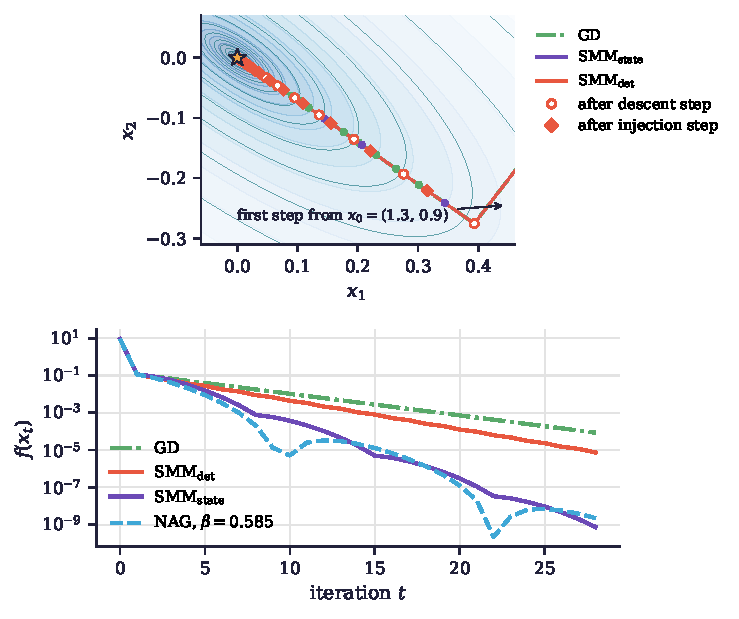
\includegraphics[width=\textwidth]{figures/ch6_trajectory.pdf}
  \caption{\smmdet\ on a tilted two dimensional quadratic with $\kappa=8$ and
  step $1/L$. Top: contours and the first iterates of gradient descent,
  \smmdet\ and \smmstate; open circles mark the points reached after descent
  steps and filled diamonds those after injection steps. Bottom: objective value
  on a log scale over $28$ iterations, with every step Nesterov at the same
  $\beta$ for comparison.}
  \label{fig:ch6:traj}
\end{figure}

\subsection{What the method needs}

\smmdet\ requires the smoothness constant $L$, for the step size, and nothing
else. Heavy ball and Nesterov\index{Nesterov acceleration} in their textbook strongly convex tunings need
both $L$ and $\mu$. The fixed momentum\index{momentum} baselines of \cref{chap:noise} need $L$
and a chosen $\beta$, and the point of the structural derivation is that SMM
does not leave that choice to the user. Memory cost is one extra vector, the
previous iterate, the same as for heavy ball\index{heavy ball} and Nesterov and less than for
adaptive methods such as Adam, which keep two moment vectors.

\section{Candidate fixed momenta}\label{sec:ch6:candidates}

The value $0.585$ is one of several natural fixed coefficients.
\Cref{tab:ch6:candidates} lists the four that the experiments of
\cref{chap:noise} compare, with the condition number\index{condition number} at which each would be the
optimal Nesterov\index{Nesterov acceleration} coefficient \eqref{eq:ch6:betaopt}, namely
$\kappa=\bigl((1+\beta)/(1-\beta)\bigr)^2$, and the slow mode noise amplification
$1/(1-\beta)$ of every step momentum\index{momentum} derived in \cref{chap:noise}.

\begin{table}[t]
\centering
\caption{Candidate fixed momentum coefficients. The column $\kappa$ gives the
condition number at which $\beta$ equals the optimal Nesterov coefficient; the
last column is the slow mode variance amplification of every step momentum
relative to gradient descent.}
\label{tab:ch6:candidates}
\small\setlength{\tabcolsep}{4pt}
\begin{tabular}{llcc}
\toprule
$\beta$ & Origin & $\kappa$ where optimal & $1/(1-\beta)$\\
\midrule
$0.500$ & round number & $9.0$ & $2.00$\\
$0.585$ & $\log_2(3/2)$, Collatz and KL ratio & $14.6$ & $2.41$\\
$0.667$ & $2/3$ & $25.0$ & $3.00$\\
$0.900$ & machine learning default~\cite{kingma2015} & $361$ & $10.0$\\
\bottomrule
\end{tabular}
\end{table}

None of these is uniformly best, and the experiments confirm it: $0.585$ does
well at small $\kappa$, $0.667$ is best on a mildly ill conditioned logistic
regression, and $0.9$ wins on strongly ill conditioned quadratics.
What distinguishes $0.585$ is not performance but provenance: it is the only entry that the arithmetic of the Collatz map fixes, rather than a round number or a convention.

\section{Related work}\label{sec:ch6:related}

\paragraph{Fixed momentum methods.} SMM belongs to the tradition of inertial
first order methods that runs from Polyak's heavy ball\index{heavy ball}~\cite{polyak1964} through
Nesterov\index{Nesterov acceleration}'s accelerated gradient~\cite{nesterov1983}; Polyak's
monograph~\cite{polyak1987} remains the clearest source for their analysis on
quadratics. The ordinary differential equation view of
Su\index{Su, W.}, Boyd\index{Boyd, S.} and Cand\`es\index{Candes, E. J.@Cand\`es, E. J.}~\cite{su2016} and the high resolution refinement of
Shi\index{Shi, B.}, Du\index{Du, S. S.}, Jordan\index{Jordan, M. I.} and Su~\cite{shi2022} explain acceleration as the interplay of
an inertial term and a gradient correction.
That picture describes every step momentum with $\beta$ tending to $1$ as the step shrinks. SMM has no inertial limit: whatever the value of $\beta<1$, its continuous time limit is a first order gradient flow, because two of its steps are two gradient steps (\cref{lem:ch6:ystep}) and it carries one gradient of memory rather than a velocity (\cref{prop:ch5b:modified}).

\paragraph{Low tuning design.} A recurring theme in modern optimization is the
search for methods whose defaults work across instances. Iterate averaging in
stochastic approximation~\cite{ruppert1988,polyak1990,polyak1992} and adaptive moment methods such as
Adam~\cite{kingma2015} are two successful examples. SMM is adjacent in spirit,
but takes its fixed coefficient from a structural source instead of from an
adaptive estimate.

\paragraph{Arithmetic structure in optimization.} Number theoretic structure
enters optimization in several established ways. Fibonacci search, which
Kiefer\index{Kiefer, J.}~\cite{kiefer1953} proved minimax optimal for unimodal functions, uses
ratios of Fibonacci numbers, and in the limit the golden ratio, to place
function evaluations. Quasi Monte Carlo methods~\cite{niederreiter1992} use
low discrepancy sequences and lattice rules built from modular arithmetic to
derandomize integration and stochastic optimization. In both cases arithmetic
decides \emph{where to evaluate}. SMM differs in where the arithmetic enters:
it decides \emph{how much inertial memory to retain}, and when.

\paragraph{Switching systems.} Alternating between two linear updates is a
switched linear system, and the stability of such systems under arbitrary or
periodic switching is the subject of Liberzon\index{Liberzon, D.}'s monograph~\cite{liberzon2003}.
Periodic switching is the benign case: stability is decided by the spectral
radius of the product of the matrices over one period, and
\cref{sec:ch6:cyclic} computes that product in closed form.

\paragraph{Majorization and minimization.} The descent half of SMM is a
majorization\index{majorization} minimization step in the sense of Lange\index{Lange, K.}, Hunter\index{Hunter, D. R.} and
Yang\index{Yang, I.}~\cite{lange2000} and Hunter and Lange~\cite{hunter2004}: for $L$ smooth
$f$ the gradient step minimizes the quadratic upper bound
$f(x_t)+\nabla f(x_t)^\top(x-x_t)+\tfrac L2\|x-x_t\|^2$. Mairal\index{Mairal, J.}~\cite{mairal2015}
develops incremental versions of this principle for large scale learning.
At the level of the optimizer the MM reading supplies the descent inequality behind \cref{prop:ch5b:monotone}: \smmdet\ is the momentum MM scheme of \cref{sec:ch5b:mm}, with the majorization point extrapolated on odd iterations.
In the Collatz
setting of \cref{chap:lyapunov} the tangent line of $\log x$ bounds the increment
of the potential at every step of $T_0$, but the map is not an MM iteration in
the usual sense, and \cref{prop:mmfails} shows that the bound cannot certify
descent. That reading of the Collatz map is the origin of the name Switching
MM\index{Switching MM}.

\paragraph{Step size schedules.} The connection that turns out to matter most
is invisible in the momentum reading of the method.
Varying the step size
periodically in gradient descent on quadratics goes back to
Richardson\index{Richardson, L. F.}~\cite{richardson1911}; Young\index{Young, D.}~\cite{young1953} showed how to choose
the steps from the roots of Chebyshev\index{Chebyshev step sizes} polynomials, and Golub\index{Golub, G. H.} and
Varga\index{Varga, R. S.}~\cite{golub1961} connected these schedules to second order iterations of
heavy ball type. Much more recently Altschuler\index{Altschuler, J. M.} and Parrilo\index{Parrilo, P. A.}~\cite{altschuler2024}
showed that carefully designed nonconstant step size schedules, the silver
stepsize schedule, accelerate gradient descent on smooth convex problems beyond
what any constant step achieves. \Cref{thm:smmquad} places SMM in this family.

\section{Switching MM is a cyclic step size method}\label{sec:ch6:cyclic}

We now analyse \smmdet\ exactly. Write $G_h(x)=x-h\nabla f(x)$ for a gradient step
of length $h$. The starting observation is an identity valid for every
differentiable $f$.

\begin{lemma}[The extrapolated point is a long gradient step]\label{lem:ch6:ystep}
Let $t$ be even. Then $x_{t+1}=G_\alpha(x_t)$, and the extrapolated point at
the following odd iteration is
\begin{equation}\label{eq:ch6:ystep}
  y_{t+1} = x_{t+1}+\beta(x_{t+1}-x_t) = x_t-(1+\beta)\alpha\nabla f(x_t)
  = G_{(1+\beta)\alpha}(x_t).
\end{equation}
Consequently $x_{t+2}=G_\alpha\bigl(G_{(1+\beta)\alpha}(x_t)\bigr)$, and in the
form that exhibits the momentum\index{momentum},
\begin{equation}\label{eq:ch6:general}
  x_{t+2} = x_{t+1}-\beta\alpha\nabla f(x_t)-\alpha\nabla f(y_{t+1}).
\end{equation}
\end{lemma}

\begin{proof}
At the even iteration $t$ the update is a plain gradient step, so
$x_{t+1}-x_t=-\alpha\nabla f(x_t)$. Substituting this displacement into the
extrapolation gives $y_{t+1}=x_{t+1}-\beta\alpha\nabla f(x_t)
=x_t-(1+\beta)\alpha\nabla f(x_t)$. The odd update is
$x_{t+2}=y_{t+1}-\alpha\nabla f(y_{t+1})$, which gives both displayed forms.
\end{proof}

So the even iterates $x_0,x_2,x_4,\dots$ of \smmdet\ are \emph{exactly} every second iterate of gradient descent with the periodic step sizes $(1+\beta)\alpha,\alpha,(1+\beta)\alpha,\alpha,\dots$, whose intermediate iterates are the extrapolated points $y_{t+1}$, for any $f$.
The momentum
buffer of \smmdet\ never holds anything except the last gradient, so the
extrapolation simply lengthens that gradient step by the factor $1+\beta$. The
odd iterates $x_{t+1}$ are an observation point off this path. On a quadratic
they lie on a second cyclic path, because gradient steps commute.

\begin{theorem}[Two step equivalence on quadratics]\label{thm:smmquad}
Let $f(x)=\tfrac12x^\top Ax-b^\top x$ with $A$ symmetric positive definite and
minimizer $x^\ast=A^{-1}b$, let $\alpha>0$ and $\beta\ge0$, and let $(x_t)$ be
generated by \cref{alg:smmdet} with step $\alpha$. For every even $t\ge0$,
\begin{equation}\label{eq:ch6:twostep}
  x_{t+2} = G_{(1+\beta)\alpha}(x_{t+1}) = G_{(1+\beta)\alpha}\bigl(G_\alpha(x_t)\bigr),
\end{equation}
that is, two \smmdet\ steps from an even index are a gradient step of length
$\alpha$ followed by a gradient step of length $(1+\beta)\alpha$, and every
iterate of \smmdet\ is an iterate of this cyclic schedule. In terms of the
error $e_t=x_t-x^\ast$,
\begin{equation}\label{eq:ch6:twosteperr}
  e_{t+2} = (I-\alpha A)\bigl(I-(1+\beta)\alpha A\bigr)e_t,\qquad t\ \text{even}.
\end{equation}
\end{theorem}

\begin{proof}
For a quadratic, $\nabla f(x)=A(x-x^\ast)$, so a gradient step of any length $h$
acts on the error linearly: $G_h(x)-x^\ast=(I-hA)(x-x^\ast)$. By
\cref{lem:ch6:ystep}, for even $t$,
\begin{gather*}
  e_{t+1}=(I-\alpha A)e_t,\qquad
  y_{t+1}-x^\ast=\bigl(I-(1+\beta)\alpha A\bigr)e_t,\\
  e_{t+2}=(I-\alpha A)(y_{t+1}-x^\ast),
\end{gather*}
and therefore $e_{t+2}=(I-\alpha A)(I-(1+\beta)\alpha A)e_t$, which is
\eqref{eq:ch6:twosteperr}. The matrices $I-\alpha A$ and $I-(1+\beta)\alpha A$
are both polynomials in $A$, hence commute, so also
\[
  e_{t+2}=\bigl(I-(1+\beta)\alpha A\bigr)(I-\alpha A)e_t
  =\bigl(I-(1+\beta)\alpha A\bigr)e_{t+1},
\]
which says $x_{t+2}=G_{(1+\beta)\alpha}(x_{t+1})$. Combined with
$x_{t+1}=G_\alpha(x_t)$ this is \eqref{eq:ch6:twostep}. By induction on even
$t$, starting from $x_0$, every iterate of \smmdet\ is an iterate of gradient
descent with steps $\alpha,(1+\beta)\alpha,\alpha,(1+\beta)\alpha,\dots$.
\end{proof}

The same fact can be seen through the state space description that
the switching systems literature would use. Restricted to an eigenvector of $A$
with eigenvalue $\lambda$, and writing $a=\alpha\lambda$, the state
$(e_t,e_{t-1})$ evolves by the descent matrix $D$ on even steps and the
Nesterov\index{Nesterov acceleration} matrix $N$ on odd steps, where
\[
  D=\begin{pmatrix}1-a&0\\1&0\end{pmatrix},\qquad
  N=\begin{pmatrix}(1-a)(1+\beta)&-(1-a)\beta\\1&0\end{pmatrix}.
\]
The product over one period is
\[
  ND=\begin{pmatrix}(1-a)(1-(1+\beta)a)&0\\1-a&0\end{pmatrix},
\]
a matrix of rank one with eigenvalues $0$ and $(1-a)(1-(1+\beta)a)$. The zero
eigenvalue records that the descent step forgets $e_{t-1}$, which is why the
period map involves only $e_t$.

\subsection{Consequences}

Write
\begin{equation}\label{eq:ch6:rho}
  \rho(a)=(1-a)\bigl(1-(1+\beta)a\bigr)=1-(2+\beta)a+(1+\beta)a^2
\end{equation}
for the two step multiplier on an eigendirection with $a=\alpha\lambda$.

\begin{corollary}[Two step contraction]\label{cor:ch6:contraction}
Under the hypotheses of \cref{thm:smmquad}, for even $t$,
\[
  \|e_{t+2}\|\le\max_{\lambda\in\operatorname{spec}(A)}|\rho(\alpha\lambda)|\;\|e_t\|,
\]
with equality for a suitable $e_t$. The per step contraction factor on an
eigendirection is $|\rho(a)|^{1/2}$.
\end{corollary}

\begin{proof}
The matrix in \eqref{eq:ch6:twosteperr} is symmetric with eigenvalues
$\rho(\alpha\lambda)$, so its operator norm is the largest of their absolute
values, attained on the corresponding eigenvector.
\end{proof}

\begin{corollary}[Stability]\label{cor:ch6:stability}
Let $0\le\beta<1$. Then $|\rho(a)|<1$ if and only if
$0<a<(2+\beta)/(1+\beta)$. In particular \smmdet\ converges linearly on every
strongly convex quadratic whenever $\alpha\le1/L$, and in fact whenever
$\alpha L<(2+\beta)/(1+\beta)$. For all $a>0$,
$\rho(a)\ge1-(2+\beta)^2/(4(1+\beta))$, a minimum attained at
$a=(2+\beta)/(2(1+\beta))$.
\end{corollary}

\begin{proof}
From \eqref{eq:ch6:rho}, $\rho(a)<1$ if and only if $a\bigl((1+\beta)a-(2+\beta)\bigr)<0$,
that is $0<a<(2+\beta)/(1+\beta)$. The condition $\rho(a)>-1$ reads
$(1+\beta)a^2-(2+\beta)a+2>0$; the discriminant of this quadratic in $a$ is
$(2+\beta)^2-8(1+\beta)=\beta^2-4\beta-4$, which is negative for $0\le\beta<1$,
so the inequality holds for every $a$. The minimum of the convex quadratic
$\rho$ is at its vertex.
\end{proof}

At $\beta=\lt-1$ the stability limit is $(2+\beta)/(1+\beta)=1+\log_3 2=1.631$
and the minimum of $\rho$ is $-0.054$, attained at $a=0.815$. The multiplier
vanishes at $a=1/(1+\beta)=0.631$ and at $a=1$: those eigendirections are
annihilated in one period.

\begin{corollary}[Slow modes]\label{cor:ch6:slow}
As $a\to0$, $\rho(a)=1-(2+\beta)a+O(a^2)$, and the per step contraction factor
is $1-\tfrac{2+\beta}{2}a+O(a^2)$. Thus in the slow directions \smmdet\ behaves
like gradient descent with the effective step
\[
  m_{\mathrm{SMM}}\,\alpha,\qquad m_{\mathrm{SMM}}=\frac{2+\beta}{2}=1.2925
  \quad\text{at }\beta=\lt-1.
\]
\end{corollary}

\begin{proof}
Expand \eqref{eq:ch6:rho} and take the square root.
\end{proof}

The effective step is just the average of the two step lengths $\alpha$ and
$(1+\beta)\alpha$, as it must be for a cyclic schedule in the slow modes. For
comparison, every step momentum\index{momentum} at fixed $\beta$, heavy ball\index{heavy ball} or Nesterov\index{Nesterov acceleration}, has
in the overdamped slow regime a real dominant root $1-a/(1-\beta)+O(a^2)$, so its
effective step multiplier is
\[
  m_{\mathrm{HB}}=m_{\mathrm{NAG}}=\frac1{1-\beta}=2.409\quad\text{at }\beta=\lt-1,
\]
and $m=10$ at $\beta=0.9$. On a $\kappa$ conditioned quadratic with $\alpha=1/L$
the slowest mode has $a=1/\kappa$, so the iteration count of \smmdet\ is of
order $\kappa/m_{\mathrm{SMM}}$: SMM is \emph{not} an accelerated method. It
improves the constant of gradient descent by about $29$ percent and is slower
than every step momentum at the same $\beta$ by the factor
$m_{\mathrm{NAG}}/m_{\mathrm{SMM}}=2.409/1.2925=1.86$ in the slow modes.
The frequency ablation of \cref{chap:noise} measures $32.85$ against $16.45$ iterations at $\kappa=10$, a ratio of $2.00$, close to this prediction.
At $\kappa=100$ it reports $293$ against $167$, a ratio of $1.75$, but that parity count is censored by the horizon $T=300$ of the experiment: $14$ of the $20$ parity runs have not reached the tolerance by $T$, and continued to convergence the parity schedule needs $318$ iterations, a ratio of $1.90$. A rerun of the same experiment with $200$ replicates (script \texttt{ch6\_ablation.py}) gives nearly the same censored means and leaves about two thirds of the parity runs short of the tolerance at $T$; run to convergence, the parity schedule needs about $315$ iterations against $166$, again a ratio of $1.90$, close to the prediction.

\subsection{Comparison with every step Nesterov}

\Cref{fig:ch6:contraction} plots the per step contraction factor against $a$
for gradient descent, every step Nesterov\index{Nesterov acceleration} at $\beta=0.585$ and $\beta=0.9$,
and \smmdet. Selected values are collected in \cref{tab:ch6:rates}. Every step
Nesterov has characteristic polynomial $z^2-(1-a)(1+\beta)z+(1-a)\beta$; its
roots are complex, with modulus $\sqrt{(1-a)\beta}$, as soon as
$(1-a)(1+\beta)^2<4\beta$, which at $\beta=0.585$ means $a>0.069$. In that
underdamped region the comparison with \smmdet\ is explicit:
$|\rho(a)|^{1/2}<\sqrt{(1-a)\beta'}$ for Nesterov with coefficient $\beta'$ if
and only if $1-(1+\beta)a<\beta'$, that is
\[
  a>\frac{1-\beta'}{1+\beta},
\]
when $(1+\beta)a\le1$; when $(1+\beta)a>1$ the condition is $(1+\beta)a-1<\beta'$, which for $\beta'=\beta$ holds for every $a<1$.
With $\beta'=\beta=0.585$ the crossover is at
$a=0.262$, and with $\beta'=0.9$ at $a=0.063$. Against gradient descent,
\smmdet\ contracts faster for every $a<2/(2+\beta)=0.774$.

\begin{figure}[t]
  \centering
  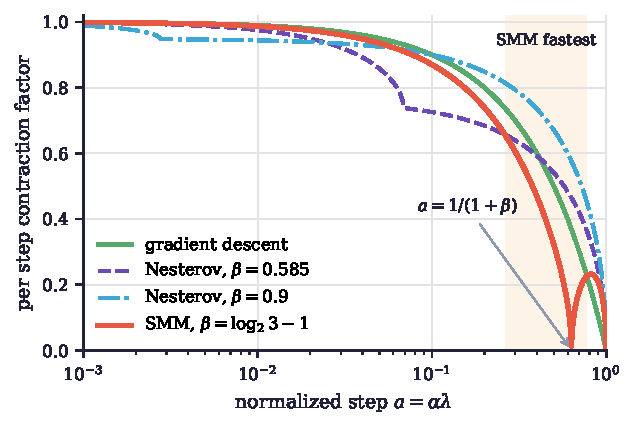
\includegraphics[width=\textwidth]{figures/ch6_contraction.pdf}
  \caption{Per step contraction factor on an eigendirection against
  $a=\alpha\lambda$ (log scale) for gradient descent, every step Nesterov at
  $\beta=0.585$ and $\beta=0.9$, and \smmdet. For \smmdet\ the factor is
  $|(1-a)(1-(1+\beta)a)|^{1/2}$; it vanishes at $a=1/(1+\beta)$ and $a=1$. SMM
  contracts fastest of the four for $0.262<a<0.774$ and is beaten by every step
  momentum in the slow modes.}
  \label{fig:ch6:contraction}
\end{figure}

\begin{table}[t]
\centering
\caption{Per step contraction factor on an eigendirection, $\beta=0.585$ unless
stated. Values computed from the characteristic roots.}
\label{tab:ch6:rates}
\begin{tabular}{ccccc}
\toprule
$a=\alpha\lambda$ & GD & NAG, $\beta=0.585$ & NAG, $\beta=0.9$ & \smmdet\\
\midrule
$0.01$ & $0.9900$ & $0.9754$ & $0.9439$ & $0.9871$\\
$0.04$ & $0.9600$ & $0.8920$ & $0.9295$ & $0.9482$\\
$0.10$ & $0.9000$ & $0.7256$ & $0.9000$ & $0.8703$\\
$0.25$ & $0.7500$ & $0.6624$ & $0.8216$ & $0.6729$\\
$0.50$ & $0.5000$ & $0.5408$ & $0.6708$ & $0.3221$\\
\bottomrule
\end{tabular}
\end{table}

The picture is consistent with the experiments.
On very well conditioned problems every $a=\alpha\lambda$ lies in $[1/\kappa,1]$, and the slowest mode $a=1/\kappa$ falls in the window $0.262<a<0.774$ where \smmdet\ contracts fastest; indeed at $\kappa=2$ it is the fastest method tested.
As $\kappa$ grows the slow
modes dominate and every step momentum\index{momentum} takes over. Nothing here depends on the
Collatz origin of $\beta$; it is the algebra of the polynomial
$\rho$.

\subsection{Chebyshev steps and silver steps}

\Cref{thm:smmquad} invites comparison with the best cyclic schedule of period
two. On a quadratic with spectrum in $[\mu,L]$, the two step polynomial
$(1-h_1\lambda)(1-h_2\lambda)$ that minimizes the maximum modulus over
$[\mu,L]$ is the scaled Chebyshev\index{Chebyshev step sizes} polynomial of degree two; its roots are
\[
  \lambda_\pm=\frac{L+\mu}2\pm\frac{L-\mu}{2\sqrt2},
\]
so $h_\pm=1/\lambda_\pm$, and the worst case two step factor is
$1/T_2\bigl((\kappa+1)/(\kappa-1)\bigr)$~\cite{young1953,golub1961}. As
$\kappa\to\infty$ the ratio of the two steps tends to
$(1+1/\sqrt2)/(1-1/\sqrt2)=(\sqrt2+1)^2=5.83$, the long step approaches
$6.83/L$, and the per step factor is $1-4/\kappa+O(\kappa^{-2})$. We computed,
for example, a per step factor of $0.709$ at $\kappa=10$ and $0.9615$ at
$\kappa=100$, against $0.870$ and $0.9871$ for \smmdet\ with $\alpha=1/L$. SMM is
thus a very conservative member of the period two family: its step ratio
$1+\beta=1.585$ is fixed and its long step is short, so that the scheme is
stable with no knowledge of $\mu$. The Chebyshev schedule needs $\mu$ to place
its roots and is fragile when the estimate is wrong; this is the cyclic step\index{cyclic step sizes}
size version of the retuning problem of \cref{sec:ch6:problem}.

Periodic Chebyshev schedules of a fixed period $p$ cannot change the order of
the iteration count: since $T_p(1+2/\kappa)=1+2p^2/\kappa+O(\kappa^{-2})$, the per
step factor is $1-2p/\kappa+O(\kappa^{-2})$. Altschuler and
Parrilo~\cite{altschuler2024} showed that suitably designed nonperiodic
schedules, built recursively and involving the silver ratio $1+\sqrt2$, do
accelerate gradient descent for smooth convex optimization. We mention this only to locate SMM: it is a fixed period two
schedule and inherits the order $\kappa$ iteration count of gradient descent,
with a better constant.

\subsection{Nonquadratic objectives}

For a general $f$, \cref{lem:ch6:ystep} still says that the even iterates follow
the cyclic schedule exactly, but with the long step \emph{first}:
$x_{t+2}=G_\alpha(G_{(1+\beta)\alpha}(x_t))$. The second statement of
\cref{thm:smmquad}, that $x_{t+2}=G_{(1+\beta)\alpha}(x_{t+1})$ so that the odd
iterates also lie on a cyclic gradient path, used commutation and is only
approximately true. The defect is of third order in the step size.

\begin{proposition}[Order of the defect]\label{prop:ch6:defect}
Suppose $\nabla^2f$ is Lipschitz with constant $M$. For even $t$, with
$h=x_{t+1}-x_t=-\alpha\nabla f(x_t)$,
\begin{multline*}
  x_{t+2}-G_{(1+\beta)\alpha}(x_{t+1})\\
  =\alpha\bigl[(1+\beta)\nabla f(x_{t+1})-\beta\nabla f(x_{t+1}-h)
   -\nabla f(x_{t+1}+\beta h)\bigr],
\end{multline*}
and
\[
  \bigl\|x_{t+2}-G_{(1+\beta)\alpha}(x_{t+1})\bigr\|
  \le\frac{M}{2}\,\beta(1+\beta)\,\alpha^3\,\|\nabla f(x_t)\|^2 .
\]
The bracket vanishes identically when $\nabla f$ is affine.
\end{proposition}

\begin{proof}
By \eqref{eq:ch6:general}, $x_{t+2}=x_{t+1}-\beta\alpha\nabla f(x_t)-\alpha\nabla
f(y_{t+1})$, and $x_t=x_{t+1}-h$, $y_{t+1}=x_{t+1}+\beta h$. Subtracting
$G_{(1+\beta)\alpha}(x_{t+1})=x_{t+1}-(1+\beta)\alpha\nabla f(x_{t+1})$ gives the
displayed identity. Write $u=x_{t+1}$ and $H=\nabla^2f(u)$. Taylor's theorem with
the Lipschitz Hessian gives $\nabla f(u-h)=\nabla f(u)-Hh+r_1$ and
$\nabla f(u+\beta h)=\nabla f(u)+\beta Hh+r_2$ with $\|r_1\|\le\tfrac M2\|h\|^2$
and $\|r_2\|\le\tfrac M2\beta^2\|h\|^2$. The bracket equals $-\beta r_1-r_2$, whose
norm is at most $\tfrac M2(\beta+\beta^2)\|h\|^2$. Multiply by $\alpha$ and use
$\|h\|=\alpha\|\nabla f(x_t)\|$.
\end{proof}

We checked the exact statement numerically on a regularized logistic regression
in five dimensions: the even iterates of \smmdet\ agree with the cyclic schedule
$(1+\beta)\alpha,\alpha$ to $10^{-16}$, while the reversed order agrees only up
to a defect that shrinks with the gradient, from $0.13$ at the first period to
$2\times10^{-8}$ by the fourth. For the purposes of this book the point is
simple: on smooth problems SMM is a period two step size schedule with steps
$(1+\beta)\alpha$ and $\alpha$, observed at two different points of each period.
For $\mu$ strongly convex and $L$ smooth $f$ the same identity gives the linear rate of \cref{thm:ch5b:rate} in \cref{chap:difference}.

\begin{remark}[What the reframing changes]\label{rem:ch6:reframing}
A natural first reading describes the parity schedule as momentum\index{momentum} that is
active half the time, a buffer that is thinned. \Cref{lem:ch6:ystep} shows that
the buffer is never more than one gradient deep, so SMM carries no long memory
at all. This is the structural reason why its noise amplification, computed in
\cref{chap:noise}, stays bounded however close $\beta$ is to one: a cyclic step\index{cyclic step sizes}
size method can only amplify noise through its step lengths, and these are
bounded by $(1+\beta)\alpha<2\alpha$.
\end{remark}

\section*{Notes}

The two derivations of $\beta$ are ours; the log displacement identity is \cref{thm:stride} of
\cref{chap:lyapunov} in Syracuse form, and the Kullback\index{Kullback and Leibler divergence} and Leibler reading is
elementary. The coefficient $\log(3/2)/\log 2=\lt-1$ is the fractional part of
$\lt$, whose continued fraction\index{continued fraction} is the subject of \cref{chap:cycles}; the
present chapter uses only its numerical value.

Polyak's book~\cite{polyak1987} treats heavy ball\index{heavy ball} and Chebyshev\index{Chebyshev step sizes} iterations on
quadratics side by side, and is the best place to see why a period two cyclic
step size method and a momentum\index{momentum} method are close relatives.
For switched linear systems see
Liberzon~\cite{liberzon2003}; for MM algorithm\index{MM algorithm}s, Lange, Hunter and
Yang~\cite{lange2000} and the tutorial~\cite{hunter2004}.

\Cref{thm:smmquad}, \cref{lem:ch6:ystep} and \cref{prop:ch6:defect} are, as far as we know, new in this book, and we regard them as the correct way to think about the method.

\section*{Exercises}

\begin{exercise}
Show that $\KL(U_j\,\|\,U_{j+1})=\log\bigl((j+1)/j\bigr)$ for nested uniform distributions, and that $\KL(U_{j+1}\,\|\,U_j)=\infty$. Show that \[ \log_3 2=\KL(U_1\,\|\,U_2)/\KL(U_1\,\|\,U_3)=1/(1+\beta), \] and that $\KL(U_1\,\|\,U_3)=\KL(U_1\,\|\,U_2)+\KL(U_2\,\|\,U_3)$ is not one of the consecutive divergences. Write the stability limit $1+\log_3 2$ of \cref{cor:ch6:stability} in terms of $\beta$ alone, and explain why its expression in divergences carries no information about stability.
\end{exercise}

\begin{exercise}
For odd $n$ with $\vt(3n+1)=1$, show that $\log S(n)-\log n$ decreases to
$\log(3/2)$ and is at most $\log(5/3)$ for $n\ge3$. Relate the excess over
$\log(3/2)$ to $\varepsilon_n$ in \cref{lem:ch6:logdisp}.
\end{exercise}

\begin{exercise}
Let $0\le\beta<1$, $\beta'\in(0,1)$ and $0<a<1$. Show that every step Nesterov\index{Nesterov acceleration} with coefficient $\beta'$ is underdamped on an eigendirection if and only if $(1-a)(1+\beta')^2<4\beta'$, and that in this regime \smmdet\ has the smaller per step contraction factor if and only if $|1-(1+\beta)a|<\beta'$, that is $(1-\beta')/(1+\beta)<a<(1+\beta')/(1+\beta)$. Verify the crossovers $0.262$ and $0.063$ quoted in the text, and show that for $\beta'\ge\beta$ the upper limit is not reached by any $a<1$.
\end{exercise}

\begin{exercise}
Replace the parity schedule by injection every third step: descend at $t\equiv0,1\pmod3$ and inject at $t\equiv2\pmod3$. Show that, as in \cref{lem:ch6:ystep}, the extrapolated point is a gradient step of length $(1+\beta)\alpha$ from the previous iterate for every differentiable $f$, so that the iterates at $t\equiv0\pmod3$ follow gradient descent with the periodic steps $\alpha,(1+\beta)\alpha,\alpha$, and that the slow mode effective step multiplier is $(3+\beta)/3$. What happens if injection occurs at two consecutive steps? Show that the second extrapolated point then involves gradients at two different points.
\end{exercise}

\begin{exercise}
Take $f(x)=x^4/4$ on $\R$. Starting from $x_0=1$ with $\alpha=1/3$ and
$\beta=\lt-1$, compute two steps of \smmdet\ and compare $x_2$ with
$G_\alpha(G_{(1+\beta)\alpha}(x_0))$ and with $G_{(1+\beta)\alpha}(G_\alpha(x_0))$.
Check the bound of \cref{prop:ch6:defect} with $M=6\sup|x|$ over the relevant
interval.
\end{exercise}

\begin{exercise}
Show that the period two schedule minimizing
$\max_{\lambda\in[\mu,L]}|(1-h_1\lambda)(1-h_2\lambda)|$ has
$h_2/h_1\to(\sqrt2+1)^2$ as $\kappa\to\infty$, and that its worst case per step
factor is $1-4/\kappa+O(\kappa^{-2})$. For which $\kappa$ is the SMM ratio
$h_2/h_1=1+\beta$ optimal?
\end{exercise}
